\documentclass[conference]{IEEEtran}
\IEEEoverridecommandlockouts
% The preceding line is only needed to identify funding in the first footnote. If that is unneeded, please comment it out.
\usepackage{cite}
\usepackage{amsmath,amssymb,amsfonts}
\usepackage{algorithmic}
\usepackage{graphicx}
\usepackage{textcomp}
\usepackage{xcolor}
\def\BibTeX{{\rm B\kern-.05em{\sc i\kern-.025em b}\kern-.08em
    T\kern-.1667em\lower.7ex\hbox{E}\kern-.125emX}}
\begin{document}

\title{The Value of Forecasting: The Effect of Building Load Forecast Errors on the Performance of an Optimal Energy Management System}

\author{\IEEEauthorblockN{Michael Wood}
\IEEEauthorblockA{Energy Department\\
Politecnico di Milano\\
Milan, Italy\\
Email: michael.wood@polimi.it}
\and
\IEEEauthorblockN{Emanuele Ogliari}
\IEEEauthorblockA{Energy Department\\
Politecnico di Milano\\
Milan, Italy\\
}
%\and
%\IEEEauthorblockN{Travis Simpkins}
%\IEEEauthorblockA{muGrid Analytics\\
%Littleton, CO, USA\\
%}
\and
\IEEEauthorblockN{Sonia Leva}
\IEEEauthorblockA{Energy Department\\
Politecnico di Milano\\
Milan, Italy\\
}
}

\maketitle

\begin{abstract}
    Distributed renewable microgrids will be a crucial technology during the energy transition. Still, many vehicle-to-grid, demand response, and storage battery resources are not utilized fully to reduce consumer electric costs or support the larger grid as needed. This is due to poor integration between systems, but also because of a challenging forecasting problem that is required to be solved to achieve near-optimal unit commitment. Traditional forecasting methods and also modern machine learning algorithms are often trained and evaluated on mean squared error, which may not optimize for or predict the performance of a forecast in an optimal energy management system. This novel work constructs several different forecasts with different error distributions to study the impact on simulated optimal battery dispatch. The findings are that forecast error is most important during peak load periods and peak price periods, especially with consumer demand charges in place, and a zero-bias forecast is not necessarily advantageous. Recommendations are made to train and validate forecasting models to be effective with a downstream decision maker and not simply be optimized for a chosen error metric.
    \end{abstract}

\begin{IEEEkeywords}
forecasting, optimization, error analysis, energy management, battery dispatch
\end{IEEEkeywords}

\section{Introduction}

Energy optimization relies heavily on accurate forecasts of electric load, dynamic prices, and renewable energy generation. From large power systems to small building microgrids, peak load events or sudden drops in solar generation can be mitigated with control actions such as demand response or dispatchable generation such as energy storage. However, depending on the control action, the cost of inaction, and other variables such as market opening and closing times, forecasting is required to anticipate the changes in load or generation, for instance by having enough State of Charge (SOC) in energy storage. This forecast-response paradigm will be increasingly important as certain regions experience more extreme weather events, and renewable generation adds uncertainty to power systems and markets. 

For these reasons, errors in forecasts can significantly impact the efficiency and reliability of large and small power systems. And since forecasts are always acted upon by some downstream decision maker, a discussion of the forecast errors must also consider the decision maker. Therefore this work examines recent literature forecasting error in power systems and then simulates several statistically diverse forecasts in an optimal Energy Management System (EMS) to evaluate the effect of forecast error on the system's performance.

\subsection{Electric Load Forecasting}

Electric load forecasting is likely the oldest forecast in power systems. Long-term forecasts on the order of years were required to plan new generation and transmission infrastructure. Medium-term forecasts on the order of months were soon required to manage seasonal variations in load, especially regarding fuel storage and generator maintenance periods. In more recent times, short-term forecasts on the order of hours to a few days aided transmission operators in managing congestion and informed market participants after the re-regulation of energy markets in the latter half of the 20th century. Most recently, nowcasting on the order of minutes has become important to manage building and campus generation and loads in real-time, which don't benefit from the spatial aggregation of loads, and thus have more load variability. 

Techniques for load forecasting include traditional statistical methods such as SARIMA and modern machine learning approaches like neural networks and support vector machines. According to \cite{b1}, while statistical methods offer robustness, machine learning models provide higher accuracy due to their ability to capture nonlinear patterns in the data. However, load forecasting errors can arise from various exogenous sources, including sudden weather changes, economic activities, and random anomalies in consumer behavior. In \cite{b2} authors emphasize the importance of error decomposition, which involves breaking down the total forecast error into systematic and random components, to better understand and mitigate the sources of inaccuracies.

\subsection{Solar Power Forecasting}

Solar power forecasting involves predicting the amount of power generated by solar PV systems. The error of these forecasts is affected by factors such as cloud cover, different types and elevations of clouds, temperature, wind, and electrical or mechanical phenomena in the PV system such as cell degradation and soiling. Typically the input features to a solar prediction model include a numerical weather prediction forecast and terrestrial solar radiation estimated by a clear sky model, such as in \cite{b7}. 

Researchers in \cite{b3} demonstrated that statistical methods like ARIMA can be adapted for solar forecasting but often fall short in capturing the high variability. Instead, machine learning techniques, including ensemble methods and hybrid physically informed neural networks have shown improved performance as in \cite{b4} and \cite{b7}. Solar forecasting errors are often characterized by their dependence on weather conditions more than autocorrelation, making integration with real-time weather data critical.

\begin{figure}
    \centering
    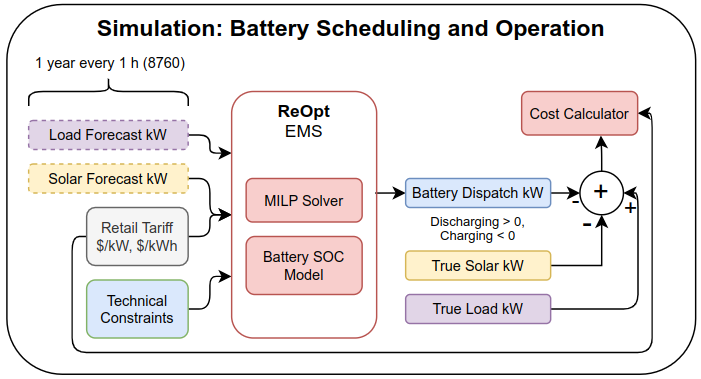
\includegraphics[width=1\linewidth]{flowchart.png}
    \caption{Simulation Flowchart. The ReOpt software is given as inputs an hourly load forecast, an hourly solar forecast, specification of the retail electric tariff, and technical constraints such as the size of the battery. The output is the hourly battery dispatch vector, which is optimal for the given inputs. The assumption is the battery dispatch vector is now directly in operation. Calculating the site load from the true load and solar vectors allows to calculate the final cost of electricity.}
    \label{fig:flowchart}
\end{figure}

% \begin{figure}
%     \centering
%     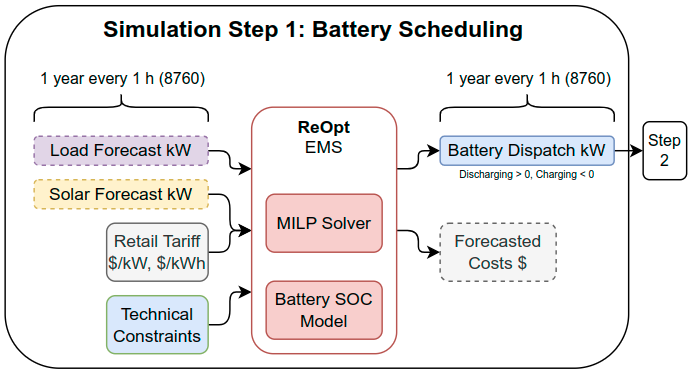
\includegraphics[width=0.95\linewidth]{step1.png}
%     \caption{Simulation Step 1. The ReOpt software is given as inputs an hourly load forecast, an hourly solar forecast, specification of the retail electric tariff, and technical constraints such as the size of the battery. The outputs are an hourly battery dispatch vector, which is optimal for the given inputs, and the associated costs that would be incurred if the load and solar vectors were true.}
%     \label{fig:step1}
% \end{figure}

\subsection{Error Analysis and Mitigation}

Error analysis involves assessing the forecast accuracy using metrics such as Mean Absolute Error (MAE), Mean Squared Error (MSE), and Mean Absolute Percentage Error (MAPE), which are most common in deterministic forecasts. In \cite{b5} authors suggest that incorporating probabilistic forecasts, which provide a range of possible outcomes instead of a single point prediction, can enhance the robustness of energy optimization strategies. Therefore probabilistic metrics are needed also, such as the Prediction Interval Coverage Probability (PICP) and Prediction Interval Normalized Average Width (PINAW). Error metrics are powerful tools for comparing forecast models and are often required for parameters fitting, and can even incorporate a benchmark prediction such as MASE, proposed in \cite{b9}.

Summary statistical metrics are helpful but often the shape of model residuals tells more of the story. A common problem is forecast bias, the tendency to have a non-zero mean for all forecasted values or just during certain intervals. This may especially occur for particular clusters of intervals with common physical phenomena, such as grid outages or extreme weather events. Extreme magnitude clusters can have a large impact on the EMS performance and be difficult to predict, especially if the events are quite rare \cite{b10}.

Mitigating forecasting errors involves both improving forecast models and developing strategies to manage uncertainty. Authors in \cite{b6} highlight the use of ensemble forecasting, where multiple models are used to generate a range of possible outcomes, thus providing a measure of the forecast uncertainty. In \cite{b6i} forecast uncertainty is mitigated with a strategy to minimize starting SOC of a hot sodium nickel battery. Additionally, reinforcement learning algorithms can continuously learn and adjust from new data can help reduce errors over time. Bayesian statistics and approaches that consider decision-making under risk may aid the final EMS or decision-maker when the uncertainty is measurable \cite{b11} 

\begin{figure}
    \centering
    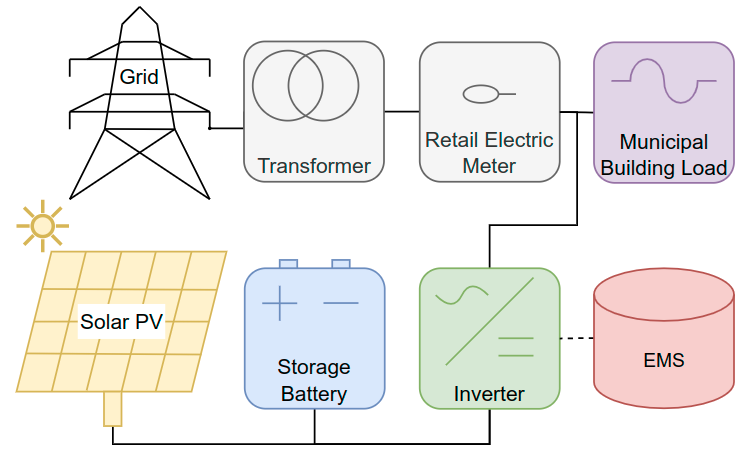
\includegraphics[width=.87\linewidth]{one-line.png}
    \caption{The simulated system is a medium-sized municipal building in Wisconsin, USA, with actual on-site solar (111 kWp). A hypothetical 100 kW 200 kWh storage battery is simulated. Load and solar forecasts are derived from true 1-minute interval data form the site. One case study includes the real retail electric tariff at this site.}
    \label{fig:one-line}
\end{figure}

% \begin{figure}
%     \centering
%     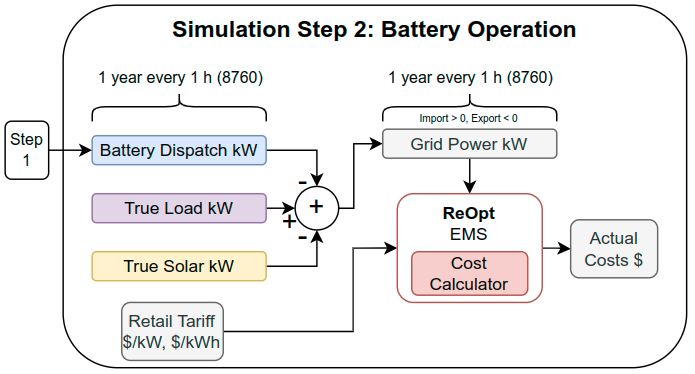
\includegraphics[width=0.95\linewidth]{step2.png}
%     \caption{Simulation Step 2. The output battery dispatch vector is used, along with the true load and solar vectors, to calculate the grid exchange vector. This is then used to calculate what the actual retail electric cost would be if the battery had been dispatched according to the output from ReOpt.}
%     \label{fig:step2}
% \end{figure}

This paper aims to construct several statistically different electric load forecasts and simulate the performance of an optimal EMS. The EMS controls a storage battery to minimize the retail cost of electricity to a medium-sized municipal building. By keeping the MAE constant among almost all the forecasts, the differing final retail costs illustrate how the shape of forecast errors impacts the downstream decision-maker in specific ways.

Our main contribution to the literature is the novel approach of manually adding disturbances to the perfect forecast to create and study specific error distributions. The methodology is robust due to the use of true measured 1-minute interval electric load, true measured 1-minute solar PV production, a thoroughly validated optimal EMS (ReOpt by the National Renewable Energy Lab) \cite{b12}, a true retail electric tariff, and two modified tariffs to study the effects of price structures on the results. Simulation code and data are published on GitHub for reproducibility.

The rest of the paper is organized as follows. In Methodology, the approach is described in detail. Next in Case Studies the specific problem and context are explained including data. Next Results are presented and discussed. And finally, Conclusions are drawn including the next steps for future work.

\section{Methodology}

\subsection{ReOpt Simulations}

The study approach is a series of computer simulations. Each simulation consists of two steps, graphically depicted in Figure \ref{fig:flowchart}. Each simulation is performed on one year of time series data, solving the unit commitment problem for a behind-the-meter electric load, co-located solar photovoltaic (PV), and a co-located storage battery. The only controllable asset is the storage battery, which can charge or discharge in any time step within its technical limits of maximum power and SOC. When the perfect load forecast (true measured load) and perfect solar forecast (true measured solar) are simulated, the result is the theoretical optimal battery dispatch for that year of load and solar measurements. The following are some useful definitions:

\begin{itemize}
    \item Load consumption: $ L(i) \in \mathbb{R}_0^+ [kW]$
    \item Solar production: $ S(i) \in \mathbb{R}_0^+ [kW]$ 
    \item Battery net, charge, and discharge: $ B(i) \in \mathbb{R}  = B_{d}^+ - B_{c}^+ [kW]$
    \item Net load: $ L_{net} = L - S$
    \item Site load: $ L_{site} = L - S - B$
    \item True measured value: $ y_t(i) \in \mathbb{R}_0^+ $
    \item Forecasted value: $ y_f(i) \in \mathbb{R}_0^+ $
    \item Error: $ \epsilon \in \mathbb{R} = y_f - y_t $
    \item Time series interval: $ \Delta t \in \mathbb{R}^+ [h] $
\end{itemize} 

If instead an imperfect load and solar forecast are provided, the result is the optimal battery dispatch given those inputs. In other words, the simulation finds a global minimum of retail electric cost believing the forecasted load and solar to be true. The simulation chooses the optimal battery dispatch given the forecasts and other inputs provided. Assuming that the battery dispatch is not modified by the EMS in the presence of true measurements, the imperfect forecasts result in a retail electric cost which is necessarily greater than or equal to the theoretical optimal given perfect forecasting.

ReOpt is a techno-economic distributed energy resource (DER) optimization tool, which is both free and open source, and is well validated in the literature \cite{b13}. It performs optimal operation and sizing of DERs, although it is not intended as a real-time optimal EMS. However, to optimally size DERs it must solve the unit commitment problem for one to several dispatchable DERs, which is the central task of an EMS. It does so by constructing and solving a mixed-integer linear program (MILP) which minimizes the life cycle cost of new and existing DERs from the perspective of the behind-the-meter DER owner. Binary decision variables are required, for instance, to prevent the battery from charging and discharging in the same time step. Depending somewhat on the particular solver used, optimality of the solution is guaranteed for moderate complexity problem formulations due to a convex cost function and continuously differentiable, linear constraints \cite{b14}. The tool is written using the JuMP library in the Julia programming language, but in this work the tool is accessed via web API and Python script.

\subsection{Forecast Construction}

\begin{table}
    \centering
    \caption{Forecasts and Two Benchmarks}
    \label{tab:forecasts}
    \setlength{\tabcolsep}{3pt}
    %\begin{tabular}{@{}p{0.4cm} @{}p{2cm} l l l l l@{}}
    %\begin{tabular}{@{}p{3cm} @{}p{5cm}}
    \begin{tabular}{l l l}
        \hline
        Error Description       & Forecast                    & nMAE  \\
        \hline
        \hline
        Perfect                 & (1) \(y_{perfect} = y_t\)           & 0.0    \\
        \hline
        Constant                & (2a) \(y_f = y_t + k\)      & 0.1   \\
                                & (2b) \(y_f = y_t - k\)      & 0.1   \\
        \hline
        Linear                  & (3a) \(y_f = y_t + ky_t\)   & 0.1   \\
                                & (3b) \(y_f = y_t - ky_t\)   & 0.1   \\
        \hline
        Quadratic               & (4a) \(y_f = y_t + ky_t^2\) & 0.1   \\
                                & (4b) \(y_f = y_t - ky_t^2\) & 0.1   \\
        \hline
        Energy (Prices)         & (5a) \(y_f = y_t + kp_e\)   & 0.1   \\
                                & (5b) \(y_f = y_t - kp_e\)   & 0.1   \\
        \hline
        Demand (Prices)         & (6a) \(y_f = y_t + kp_d\)   & 0.1   \\
                                & (6b)\(y_f = y_t - kp_d\)    & 0.1   \\
        \hline
        Random (Gaussian)       & (7) \(y_f = y_t + X\)       & 0.1   \\
        \\
        \hline
        Persistence             & (8) \(y_{persist} = y_t(i-168)\)    & 0.033 \\
        \hline
        \hline
        Solar Only (no battery) & (9) No forecast             & n/a   \\
        \hline
    \end{tabular}
\end{table}

Rather than train various traditional and machine learning models to predict a time series, in this work the forecasts are manually manipulated starting from the true time series. In this way, the shape of the forecast error can be controlled and the effect on the EMS performance can be studied. 

\begin{enumerate}
\item One hypothesis is that errors during peak load periods is especially harmful to the EMS performance, especially when the rate tariff contains a price on peak demand, also called a demand charge.

\item A second hypothesis is that forecast errors during high energy prices is detrimental to EMS performance, especially in the absence of a demand charge.
\end{enumerate}

These hypotheses can be tested by manipulating the original load vector, which is a perfect forecast, with a disturbance that is proportional to the load magnitude, the load magnitude squared, energy prices, or demand prices. Table \ref{tab:forecasts} summarizes these constructed forecasts in rows 2 through 7, which are referenced as forecasts 2a through 7. Additionally, there is forecast 8 which is a seasonal persistence forecast where the lag value equals one week.

\begin{align}
    \text{nMAE } [\frac{kW}{kW}] = \frac{1}{N} \sum_{i=1}^N \frac{|y_f - y_t|}{max(y_t)} \label{eq:nmae} 
\end{align} 

A linear scaling factor $k$ is fit and applied separately to each forecast such that the normalized mean absolute error (nMAE) of each forecast is exactly 0.10. The value of 0.10 was determined experimentally to show a good spread of results: with an nMAE too low all the forecasts would be nearly perfect and indistinguishable, and vice versa.  The exceptions are that a perfect forecast will have an nMAE of zero, and a seasonal persistence forecast is possibly more interesting without other disturbances since it is already a good benchmark forecast \cite{b9}. By forcing all the manipulated forecasts to have the same nMAE, any differences in the EMS performance can be attributed to the shape of the error distribution and not just the magnitude.

Because there are no regression or machine learning models to fit we don't separate the data into train, validation, and test subsets.

\subsection{Performance Evaluation}

A premise of this work is that the utility of a distributed energy forecast should be determined by how much it reduces the final retail electric cost compared to a benchmark. The operational electric cost here is defined as what a customer would pay on a bill, less any fixed charges and particularly difficult-to-model components of the tariff, such as the rolling annual demand charge. Revenue from selling extra solar energy to the grid will be represented as a negative cost. Each timestep in $L_{site}$ belongs to exactly one time-of-use (TOU) period from 1 to $K$. Then each TOU period is assigned an energy buy price, demand charge price, and energy sell price. Equation \ref{eq:cost} calculates the dot product of in-TOU-period site loads and prices for each period, as well as the maximum monthly site load for each TOU period, which is multiplied by the TOU period's associated demand charge.

\begin{align}
    C_t,m           & = \sum_{k=1}^K [p_{d,k,m}  max(L^+_{site,k,m})  \notag \\
                & + p_{e,k,m} \sum (L^+_{site,k,m}\Delta t)  \notag \\
                & + p_{s,k,m} \sum (L^-_{site,k,m}\Delta t) ] \label{eq:cost} \\
                 \text{subject to:}&  \notag \\
                L_{site,k,m}^+(i) & \ge 0 \text{ and } L_{site,k,m}^-(i) \le 0\ \forall\ i \notag \\
%\end{align}
%\begin{align*}
                \text{where:}& \notag \\
                k & \text{: TOU period} \notag \\
                K & \text{: total TOU periods} \notag \\
                m & \text{: month} \notag \\
    C_t,m         & \in \mathbb{R}^+ [\$] \text{: total monthly retail electric cost} \notag \\
    p_{x,k,m}     & \in \mathbb{R}^+ [\$/kW] \text{ or } [\$/kWh] \text{: price for TOU } k \notag 
\end{align}

\begin{table}
    \centering
    \caption{Retail Electric Tariff}
    \label{tab:tariff}
    \setlength{\tabcolsep}{3pt}
    %\begin{tabular}{@{}p{0.4cm} @{}p{2cm} l l l l l@{}}
    %\begin{tabular}{@{}p{3cm} @{}p{5cm}}
    \begin{tabular}{l l l l l}
        \hline
        Period & Hours & Buy Prices & Buy Prices & Sell Price  \\
         &  & (Jun 1 - Sep 30) & (Oct 1 - May 31) & (all months) \\
        \hline
        \hline
        Off peak & 0:00-9:00,  & 0.056 \$/kW  & 0.056 \$/kW & 0.050 \$/kWh \\
                  & 21:00-0:00 &              &        &       \\
        \hline
        Peak     & 9:00-21:00   & 0.075 \$/kWh, & 0.070 \$/kWh, & 0.050 \$/kWh \\
                 &              & 13 \$/kW & 11 \$/kW & \\
        \hline
    \end{tabular}
\end{table}

\begin{table}
    \centering
    \caption{Case Studies}
    \label{tab:case-studies}
    \setlength{\tabcolsep}{3pt}
    %\begin{tabular}{@{}p{0.4cm} @{}p{2cm} l l l l l@{}}
    %\begin{tabular}{@{}p{3cm} @{}p{5cm}}
    \begin{tabular}{l l l}
        \hline
        & Tariff & Modifications \\
        \hline
        \hline
        1 & Retail Electric Tariff (Table \ref{tab:tariff}) & \\
        2 & Retail Electric Tariff (Table \ref{tab:tariff}) & All \$/kW prices = 0  \\
        3 & Retail Electric Tariff (Table \ref{tab:tariff}) & Sell price = CA NEM3.0 \\
        \hline
    \end{tabular}
\end{table}

The two benchmarks in Table \ref{tab:forecasts} are forecast 1, the perfect forecast, and forecast 9, a solar-only benchmark, which has no battery. With no controllable DERs there are no decision variables and no forecasting to be done. The perfect forecast is a theoretical optimal (lowest cost) that can't be exceeded. The solar-only case should represent a low benchmark: an optimal EMS controlling a battery should be able to perform better than if the battery wasn't there at all.  

\begin{align}
    P(C_x) [\frac{kW}{kW}]= & (C_x - C_{x,perfect}) \over (C_{x,solar-only} - C_{x,perfect}) \label{eq:performance} \\
    \text{where:}& \notag \\
    x  \in & \{e:\text{energy},d:\text{demand},r:\text{revenue},t:\text{total} \}  \notag \\
    C_x =& \text{ cost of forecast to be evaluated [\$]}  \notag \\
    C_{x,perfect} =& \text{ cost of perfect forecast [\$]}  \notag \\
    C_{x,solar-only} =& \text{ cost of solar-only benchmark [\$]}  \notag 
\end{align} 

These two book-end benchmarks suggest a normalized performance metric where a sample cost value $C$ lies in the range between the perfect forecast (1) and solar-only benchmark (9). This "performance" $P$ takes a value of 0 when the forecast cost is equal to the solar-only benchmark and a value of 1 when the forecast cost equals the theoretical optimal.

\section{Case Studies}

\begin{figure}
    \centering
    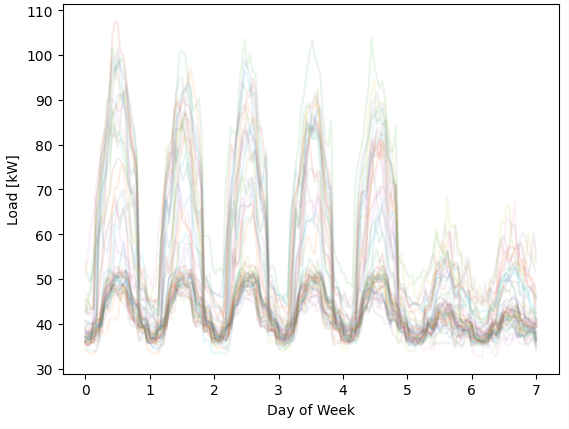
\includegraphics[width=0.95\linewidth]{weekly.png}
    \caption{The municipal building load overlaid weekly shows the daily seasonality, weekly seasonality, and much larger peaks which we confirm elsewhere to be during the summer months, and likely due to increased occupancy and air conditioning. }
    \label{fig:data-weekly}
\end{figure}



Three case studies are presented in Table \ref{tab:case-studies}, each with a different tariff structure, but all with the same forecasts, benchmarks, and simulated DERs and site. The base tariff in Table \ref{tab:tariff} is only slightly simplified compared to the in vivo one, due to limitations of ReOpt in including a rolling annual demand charge on the cost function. This would only add marginally to the demand cost: 0.056 \$/kW compared to 11 and 13 \$/kW for Winter and Spring, respectively. In the second case study all demand charges are zeroed to see how errors affect the EMS in two very different objective functions: the first with a strong incentive to shave peaks, and the second not. In the third case study the demand charges are left intact but instead of a fixed solar sellback price of 0.05 \$/kWh, the California NEM3.0 price is used, which is a time-varying price based on the wholesale market price. Due to the famous duck curve and the need for late summer evening generation, prices in NEM3.0 can reach over 3 \$/kWh.

In all three case studies only the load forecast is manipulated according to Table \ref{tab:forecasts}. Since solar PV has zero marginal cost it is always dispatched except for technical reasons for curtailment. Therefore the unit commitment problem can be reframed not as dispatching solar PV and storage to minimize the cost of electricity incurred by the load, but instead as dispatching only storage to minimize the cost of net load ($load - solar$, where $load$ and $solar \in \mathbb{R}_0^+$). Now a positive error in the load forecast is identical to a negative error in the solar forecast, and vice versa. Furthermore, the combination of a load positive error and solar negative error can be reframed as the combined magnitude error in the net load.  

The nMAE of all forecasts is equal to 0.10 except the perfect forecast which is 0, seasonal persistence which is 0.033, and the solar-only benchmark which has no forecast.

The site in the case studies is a medium-sized municipal building in northern Wisconsin, USA. The site has previously installed solar PV and energy meters which capture 1-minute time series data. For the purpose of this study the battery and EMS are just abstractions. The simulations should somewhat accurately model power flows and battery charge and discharge of the site in Figure \ref{fig:one-line}. Conductor and transformer losses are estimated as a constant loss percentage, and real power reduction due to fluctuating power factor is not considered. 

\begin{figure}
    \centering
    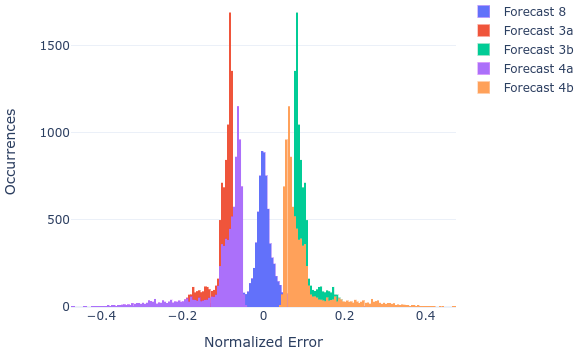
\includegraphics[width=1\linewidth]{hist.png}
    \caption{Error Distributions of Several Forecasts. The Persist errors are well-behaved with a zero mean, as expected for a differences seasonal time series. The Linear and Quad errors have substantial skew and then long tails away from zero, and the positive and negative bias forecasts are mirror images, as expected. The Quad forecast errors appear to have still more skew.}
    \label{fig:hist}
\end{figure}

\begin{figure}
    \centering
    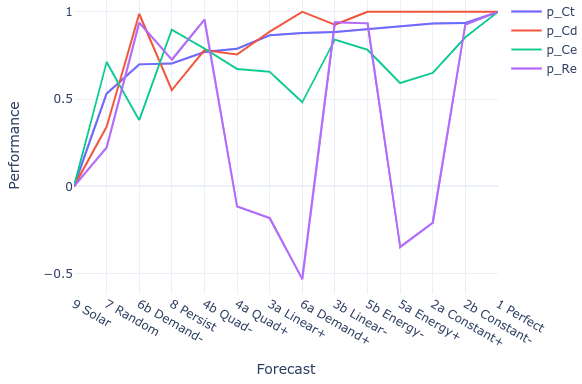
\includegraphics[width=1\linewidth]{perf_lines.png}
    \caption{Case Study 1 Performance. The horizontal axis is sorted for increasing total cost performance $P_{Ct}$ which rises quickly above 0.5. Some forecasts have a negative performance on revenue despite a good total cost performance. This is the same data as in Table \ref{tab:performance}.}
    \label{fig:perf-lines}
\end{figure}

\begin{figure}
    \centering
    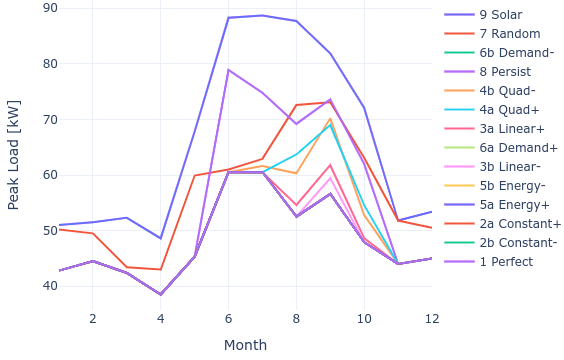
\includegraphics[width=1\linewidth]{monthly_peaks_lines.png}
    \caption{Case Study 1 Monthly Peaks by Forecast. For this case study demand cost is a good predictor of total cost. Some forecasts such as 2a and 2b are able to chase down demand peaks for all months, whereas others are less able especially in August, September, and October. }
    \label{fig:monthly-peaks-lines}
\end{figure}


\section{Results}

The error distributions in Figure \ref{fig:hist} reflect the intention to have different positive and negative forecast biases and to cluster the errors near peak values. In the 2a and 2b Constant forecasts the errors take a single positive or negative value to the constant positive or negative offset (not shown in the image).

The final calculated costs for case study 1 in Figure \ref{fig:perf-lines} (sorted in order of increasing $P_{Ct}$) show that demand cost $P_{Cd}$ is a good predictor of total cost. In fact, the Pearson correlation between the two is 0.94, whereas energy cost $P_{Ce}$ only correlates at 0.74 and revenue $P_{Re}$ is uncorrelated at 0.14. The Constant and Energy price forecasts are likely the best performing because both have fairly evenly distributed errors throughout the day, whereas Linear, Demand, and Quadratic forecasts focus the errors around load peaks or high demand prices. An unexpected finding is that the worst-performing constructed forecast is the Random gaussian disturbance. Any single timestep can set the demand peak of the month. It appears that the randomly meandering forecast, coupled with a load time series that routinely rises to near its monthly peak (Figure \ref{fig:data-weekly}), spells disaster for an EMS charged with always shaving peaks.

This is confirmed by case study 3 results, also deriving from a demand charge tariff, in Table \ref{tab:performance} where the Random forecast is again the worst performer. Both case studies 1 and 3 have the same four forecasts near or above 0.90: 2b Constant-, 2a Constant+, 5b Energy-, and 3b Linear-. Both case studies also have similar low performers: Random, Persist, and 6b Demand-, and in both forests the positive and negative bias forecasts don't show obvious trends.

\begin{table}%[!ht]
    \centering
    \caption{Case Study 1: Forecasts vs Retail Electric Cost}
    \label{tab:cs1-cost}
    \begin{tabular}{l l l l l}
    \hline
        ~ & $C_e [\$]$ & $C_d [\$]$ & $R_e [\$]$ & $C_t [\$]$ \\ \hline \hline
        1 Perfect & 21867.31 & 4608.50 & 8.00 & 26467.81 \\ \hline
        2b Constant- & 22256.94 & 4608.56 & 42.00 & 26823.50 \\ \hline
        2a Constant+ & 22805.10 & 4608.56 & 574.00 & 26839.66 \\ \hline
        5a Energy+ & 22959.75 & 4608.56 & 639.00 & 26929.31 \\ \hline
        5b Energy- & 22449.53 & 4608.56 & 39.00 & 27019.09 \\ \hline
        3b Linear- & 22293.84 & 4851.25 & 36.00 & 27109.09 \\ \hline
        6a Demand+ & 23256.18 & 4608.56 & 725.00 & 27139.74 \\ \hline
        3a Linear+ & 22786.99 & 4984.94 & 561.00 & 27210.93 \\ \hline
        4a Quad+ & 22742.46 & 5425.37 & 530.00 & 27637.83 \\ \hline
        4b Quad- & 22433.59 & 5340.66 & 29.00 & 27745.25 \\ \hline
        8 Persist & 22140.92 & 6105.94 & 136.00 & 28110.86 \\ \hline
        6b Demand- & 23527.14 & 4646.89 & 37.00 & 28137.03 \\ \hline
        7 Random & 22635.07 & 6810.84 & 372.00 & 29073.91 \\ \hline
        9 Solar & 24546.16 & 7951.44 & 476.00 & 32021.60 \\ \hline
    \end{tabular}
\end{table}

In case study 2 there is no demand charge, and now the energy cost $P_{Ce}$ correlates with the total cost at 0.92. Without the demand charge a forecast with errors concentrated around high demand prices should be relatively error-free during the other times of the day, and indeed the two best performing models are 6a and 6b Demand+ and Demand-. Persist performs above 0.90 for the first time and Random is 0.79, suggesting both of those error shapes are harmful to peak shaving.




% \begin{table}[!ht]
%     \centering
%     \caption{Case Study 1: Forecasts vs Performance}
%     \label{tab:cs1-performance}    
%     \begin{tabular}{l l l l l}
%     \hline
%         ~ & $P_{Ce}$ & $P_{Cd}$ & $P_{Re}$ & $P_{Ct}$ \\ \hline \hline
%         9 Solar & 0 & 0 & 0 & 0 \\ \hline
%         7 Random & 0.71 & 0.34 & 0.22 & 0.53 \\ \hline
%         6b Demand- & 0.38 & 0.99 & 0.94 & 0.70 \\ \hline
%         8 Persist & 0.90 & 0.55 & 0.73 & 0.70 \\ \hline
%         4b Quad- & 0.79 & 0.78 & 0.95 & 0.77 \\ \hline
%         4a Quad+ & 0.67 & 0.76 & -0.12 & 0.79 \\ \hline
%         3a Linear+ & 0.66 & 0.89 & -0.18 & 0.87 \\ \hline
%         6a Demand+ & 0.48 & 1.00 & -0.53 & 0.88 \\ \hline
%         3b Linear- & 0.84 & 0.93 & 0.94 & 0.89 \\ \hline
%         5b Energy- & 0.78 & 1.00 & 0.93 & 0.90 \\ \hline
%         5a Energy+ & 0.59 & 1.00 & -0.35 & 0.92 \\ \hline
%         2a Constant+ & 0.65 & 1.00 & -0.21 & 0.93 \\ \hline
%         2b Constant- & 0.85 & 1.00 & 0.93 & 0.94 \\ \hline
%         1 Perfect & 1 & 1 & 1 & 1 \\ \hline
%     \end{tabular}
% \end{table}

% \begin{table}[!ht]
%     \centering
%     \caption{Case Study 2 (No Demand Price): Forecasts vs Performance}
%     \label{tab:cs2-performance}    
%     \begin{tabular}{l l l l}
%     \hline
%         ~ & $P_{Ce}$ & $P_{Re}$ & $P_{Ct}$ \\ \hline \hline
%         9 Solar & 0 & 0 & 0 \\ \hline
%         5a Energy+ & 0.44 & -0.75 & 0.69 \\ \hline
%         5b Energy- & 0.78 & 0.93 & 0.75 \\ \hline
%         4b Quad- & 0.79 & 0.95 & 0.75 \\ \hline
%         2a Constant+ & 0.54 & -0.49 & 0.76 \\ \hline
%         3a Linear+ & 0.55 & -0.45 & 0.77 \\ \hline
%         4a Quad+ & 0.58 & -0.36 & 0.78 \\ \hline
%         7 Random & 0.67 & 0.10 & 0.79 \\ \hline
%         3b Linear- & 0.84 & 0.94 & 0.82 \\ \hline
%         2b Constant- & 0.85 & 0.93 & 0.84 \\ \hline
%         8 Persist & 0.87 & 0.65 & 0.92 \\ \hline
%         6b Demand- & 1.00 & 1.00 & 1.00 \\ \hline
%         6a Demand+ & 1.00 & 1.00 & 1.00 \\ \hline
%         1 Perfect & 1 & 1 & 1 \\ \hline
%     \end{tabular}
% \end{table}

% \begin{table}[!ht]
%     \centering
%     \caption{Case Study 3 (NEM3.0 Sell Price): Forecasts vs Performance}
%     \label{tab:cs3-performance}    
%     \begin{tabular}{l l l l l}
%     \hline
%     ~ & $P_{Ce}$ & $P_{Cd}$ & $P_{Re}$ & $P_{Ct}$ \\ \hline \hline
%         9 Solar & 0 & 0 & 0 & 0 \\ \hline
%         7 Random & 0.73 & 0.21 & 0.25 & 0.45 \\ \hline
%         8 Persist & 0.90 & 0.55 & 0.73 & 0.70 \\ \hline
%         6b Demand- & 0.37 & 0.99 & 0.89 & 0.70 \\ \hline
%         4a Quad+ & 0.67 & 0.76 & -0.12 & 0.75 \\ \hline
%         4b Quad- & 0.79 & 0.78 & 0.94 & 0.78 \\ \hline
%         6a Demand+ & 0.48 & 1.00 & -0.57 & 0.82 \\ \hline
%         3a Linear+ & 0.66 & 0.89 & -0.19 & 0.82 \\ \hline
%         5a Energy+ & 0.59 & 1.00 & -0.37 & 0.87 \\ \hline
%         3b Linear- & 0.84 & 0.93 & 0.93 & 0.89 \\ \hline
%         2a Constant+ & 0.65 & 1.00 & -0.23 & 0.89 \\ \hline
%         5b Energy- & 0.78 & 1.00 & 0.92 & 0.90 \\ \hline
%         2b Constant- & 0.85 & 1.00 & 0.92 & 0.94 \\ \hline
%         1 Perfect & 1 & 1 & 1 & 1 \\ \hline
%     \end{tabular}
% \end{table}

%%%%%%%%%%%%%%%%%%%

\begin{table}%[!ht]
    \centering
    \caption{Case Studies 1-3: Forecasts vs Performance}
    \label{tab:performance}
    \setlength{\tabcolsep}{1pt}
    \begin{tabular}{l|l l l l|l l l| l l l l}
        \hline
        ~            & CS1      &          &          &               & CS2      &          &               & CS3      &          &          &          \\ \hline 
        ~            & $P_{Ce}$ & $P_{Cd}$ & $P_{Re}$ & $P_{Ct}$      & $P_{Ce}$ & $P_{Re}$ & $P_{Ct}$      & $P_{Ce}$ & $P_{Cd}$ & $P_{Re}$ & $P_{Ct}$ \\ \hline \hline 
        9 Solar      & 0        & 0        & 0        & 0             & 0        & 0        & 0             & 0        & 0        & 0        & 0        \\ \hline  
        8 Persist    & 0.90     & 0.55     & 0.73     & 0.70          & 0.87     & 0.65     & \textbf{0.92} & 0.90     & 0.55     & 0.73     & 0.70     \\ \hline
        7 Random     & 0.71     & 0.34     & 0.22     & 0.53          & 0.67     & 0.10     & 0.79          & 0.73     & 0.21     & 0.25     & 0.45     \\ \hline
        6b Demand-   & 0.38     & 0.99     & 0.94     & 0.70          & 1.00     & 1.00     & \textbf{1.00} & 0.37     & 0.99     & 0.89     & 0.70     \\ \hline
        6a Demand+   & 0.48     & 1.00     & -0.53    & 0.88          & 1.00     & 1.00     & \textbf{1.00} & 0.48     & 1.00     & -0.57    & 0.82     \\ \hline
        5b Energy-   & 0.78     & 1.00     & 0.93     & 0.90          & 0.78     & 0.93     & 0.75          & 0.78     & 1.00     & 0.92     & \textbf{0.90}     \\ \hline
        5a Energy+   & 0.59     & 1.00     & -0.35    & \textbf{0.92} & 0.44     & -0.75    & 0.69          & 0.59     & 1.00     & -0.37    & 0.87     \\ \hline
        4b Quad-     & 0.79     & 0.78     & 0.95     & 0.77          & 0.79     & 0.95     & 0.75          & 0.79     & 0.78     & 0.94     & 0.78     \\ \hline
        4a Quad+     & 0.67     & 0.76     & -0.12    & 0.79          & 0.58     & -0.36    & 0.78          & 0.67     & 0.76     & -0.12    & 0.75     \\ \hline
        3b Linear-   & 0.84     & 0.93     & 0.94     & 0.89          & 0.84     & 0.94     & 0.82          & 0.84     & 0.93     & 0.93     & \textbf{0.89}     \\ \hline
        3a Linear+   & 0.66     & 0.89     & -0.18    & 0.87          & 0.55     & -0.45    & 0.77          & 0.66     & 0.89     & -0.19    & 0.82     \\ \hline
        2b Constant- & 0.85     & 1.00     & 0.93     & \textbf{0.94} & 0.85     & 0.93     & 0.84          & 0.85     & 1.00     & 0.92     & \textbf{0.94}     \\ \hline
        2a Constant+ & 0.65     & 1.00     & -0.21    & \textbf{0.93} & 0.54     & -0.49    & 0.76          & 0.65     & 1.00     & -0.23    & \textbf{0.89}     \\ \hline
        1 Perfect    & 1        & 1        & 1        & 1             & 1        & 1        & 1             & 1        & 1        & 1        & 1        \\ \hline
    \end{tabular}
\end{table}

%%%%%%%%%%%%%%%%%

% \begin{figure}
%     \centering
%     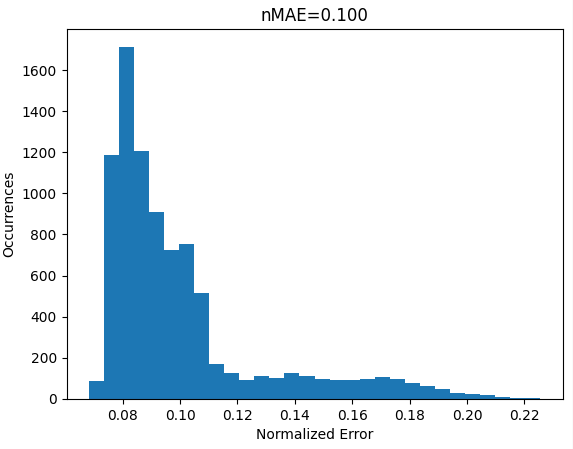
\includegraphics[width=0.95\linewidth]{hist_linscaledup.png}
%     \caption{Forecast 3+: Error $\alpha$ Load (positive). The errors have heavy skew to the low end and a long tail to the high end. This effect is mirrored for the forecast 3- for negative bias, and more pronounced for both forecast 4+ and 4- with the quadratic relationship.}
%     \label{fig:hist-linscaledup}
% \end{figure}

% \begin{figure}
%     \centering
%     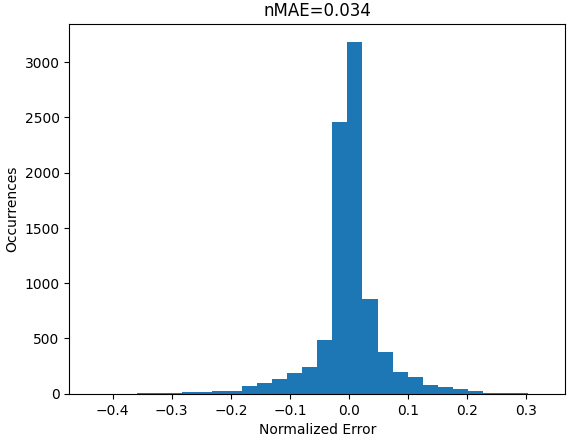
\includegraphics[width=0.95\linewidth]{hist_persist.png}
%     \caption{Forecast 8: Seasonal Persistence. Distribution of errors for the 7day persistence forecast, the only once with a lower nMAE than 0.10 (0.033).The errors are essentially the difference of the time series so we expect to see symmetry around a mean of zero.}
%     \label{fig:hist-persist}
% \end{figure}



\section{Conclusions}

Analyzing and mitigating errors in electric load and solar forecasts are crucial for optimizing energy systems because of the decision maker downstream of the forecast. The initial investigation has discovered that several different load forecasts with identical nMAE can have extremely different performances in a simulated EMS. Advances in machine learning, synthetic data, and transfer learning offers promising improvements in forecast accuracy. However ongoing research is essential to develop the right forecasts and not generic ones, especially regarding peak shaving and peak load forecasting.

Future work will include combined true error distributions from trained forecast models, and will combine solar and load forecast errors explicitly to discern if the errors often have similar properties or not. Future forecasting efforts will use tools like custom loss functions, Kalman filtering, and decision making under risk approaches to tune the forecast in the direction that is optimal for the EMS to reduce costs. Finally, the cost of carbon will be considered in a multi-objective optimization in addition to economic cost.


\begin{thebibliography}{00}

\bibitem{b1} Taylor, J. W., & McSharry, P. E. (2007). Short-term load forecasting methods: An evaluation based on European data. IEEE Transactions on Power Systems, 22(4), 2213-2219.

\bibitem{b2} Hong, T., Pinson, P., & Fan, S. (2016). Global energy forecasting competition 2012 and beyond. International Journal of Forecasting, 32(3), 896-913.

\bibitem{b3} Bacher, P., Madsen, H., & Nielsen, H. A. (2009). Online short-term solar power forecasting. Solar Energy, 83(10), 1772-1783.

\bibitem{b4} Yang, D., Kleissl, J., Gueymard, C. A., Pedro, H. T. C., & Coimbra, C. F. M. (2018). History and trends in solar irradiance and PV power forecasting: A preliminary assessment and review using text mining. Solar Energy, 168, 60-101.

\bibitem{b5} Zhang, G., Wang, J., & Zhang, W. (2018). Review on probabilistic forecasting of wind power generation. Renewable and Sustainable Energy Reviews, 32(3), 858-872.

\bibitem{b6} Pinson, P., & Kariniotakis, G. (2010). Conditional prediction intervals of wind power generation. IEEE Transactions on Power Systems, 25(4), 1845-1856.

\bibitem{b6i} Grillo, S., Marinelli, M., Massucco, S., & Silvestro, F. (2012). Optimal management strategy of a battery-based storage system to improve renewable energy integration in distribution networks. IEEE Transactions on Smart Grid, 3(2), 950-958.

\bibitem{b7} Costa, A., Crespo, A., Navarro, J., Lizcano, G., Madsen, H., & Feitosa, E. (2008). A review on the young history of the wind power short-term prediction. Renewable and Sustainable Energy Reviews, 12(6), 1725-1744.

\bibitem{b8} Leva, S., Dolara, A., Grimaccia, F., Mussetta, M., & Ogliari, E. (2017). Analysis and validation of 24 hours ahead neural network forecasting of photovoltaic output power. Mathematics and computers in simulation, 131, 88-100.

\bibitem{b9} Hyndman, R. J. (2006). Another look at forecast-accuracy metrics for intermittent demand. Foresight: The International Journal of Applied Forecasting, 4(4), 43-46.

\bibitem{b10} Cirillo, P., & Taleb, N. N. (2020). Tail risk of contagious diseases. Nature Physics, 16(6), 606-613.

\bibitem{b11} Reggiani, P., & Weerts, A. H. (2008). A Bayesian approach to decision-making under uncertainty: An application to real-time forecasting in the river Rhine. Journal of Hydrology, 356(1-2), 56-69.

\bibitem{b12} Simpkins, T., Cutler, D., Anderson, K., Olis, D., Elgqvist, E., Callahan, M., & Walker, A. (2014). REopt: a platform for energy system integration and optimization (Vol. 45875, p. V002T03+006). American Society of Mechanical Engineers.

\bibitem{b13} Mishra, S., Pohl, J., Laws, N., Cutler, D., Kwasnik, T., Becker, W., ... & Elgqvist, E. (2022). Computational framework for behind-the-meter DER techno-economic modeling and optimization: REopt Lite. Energy Systems, 13(2), 509-537.

\bibitem{b14} Ogunmodede, O., Anderson, K., Cutler, D., & Newman, A. (2021). Optimizing design and dispatch of a renewable energy system. Applied Energy, 287, 116527.

\end{thebibliography}

\end{document}
